\chapter{Experimental Results}
\label{chapter6}

\section{Overview} 

\section{Heterogeneous CSS Results}

\subsection{Hard Decision Combining}

\begin{figure}[ht!]
	\centering
	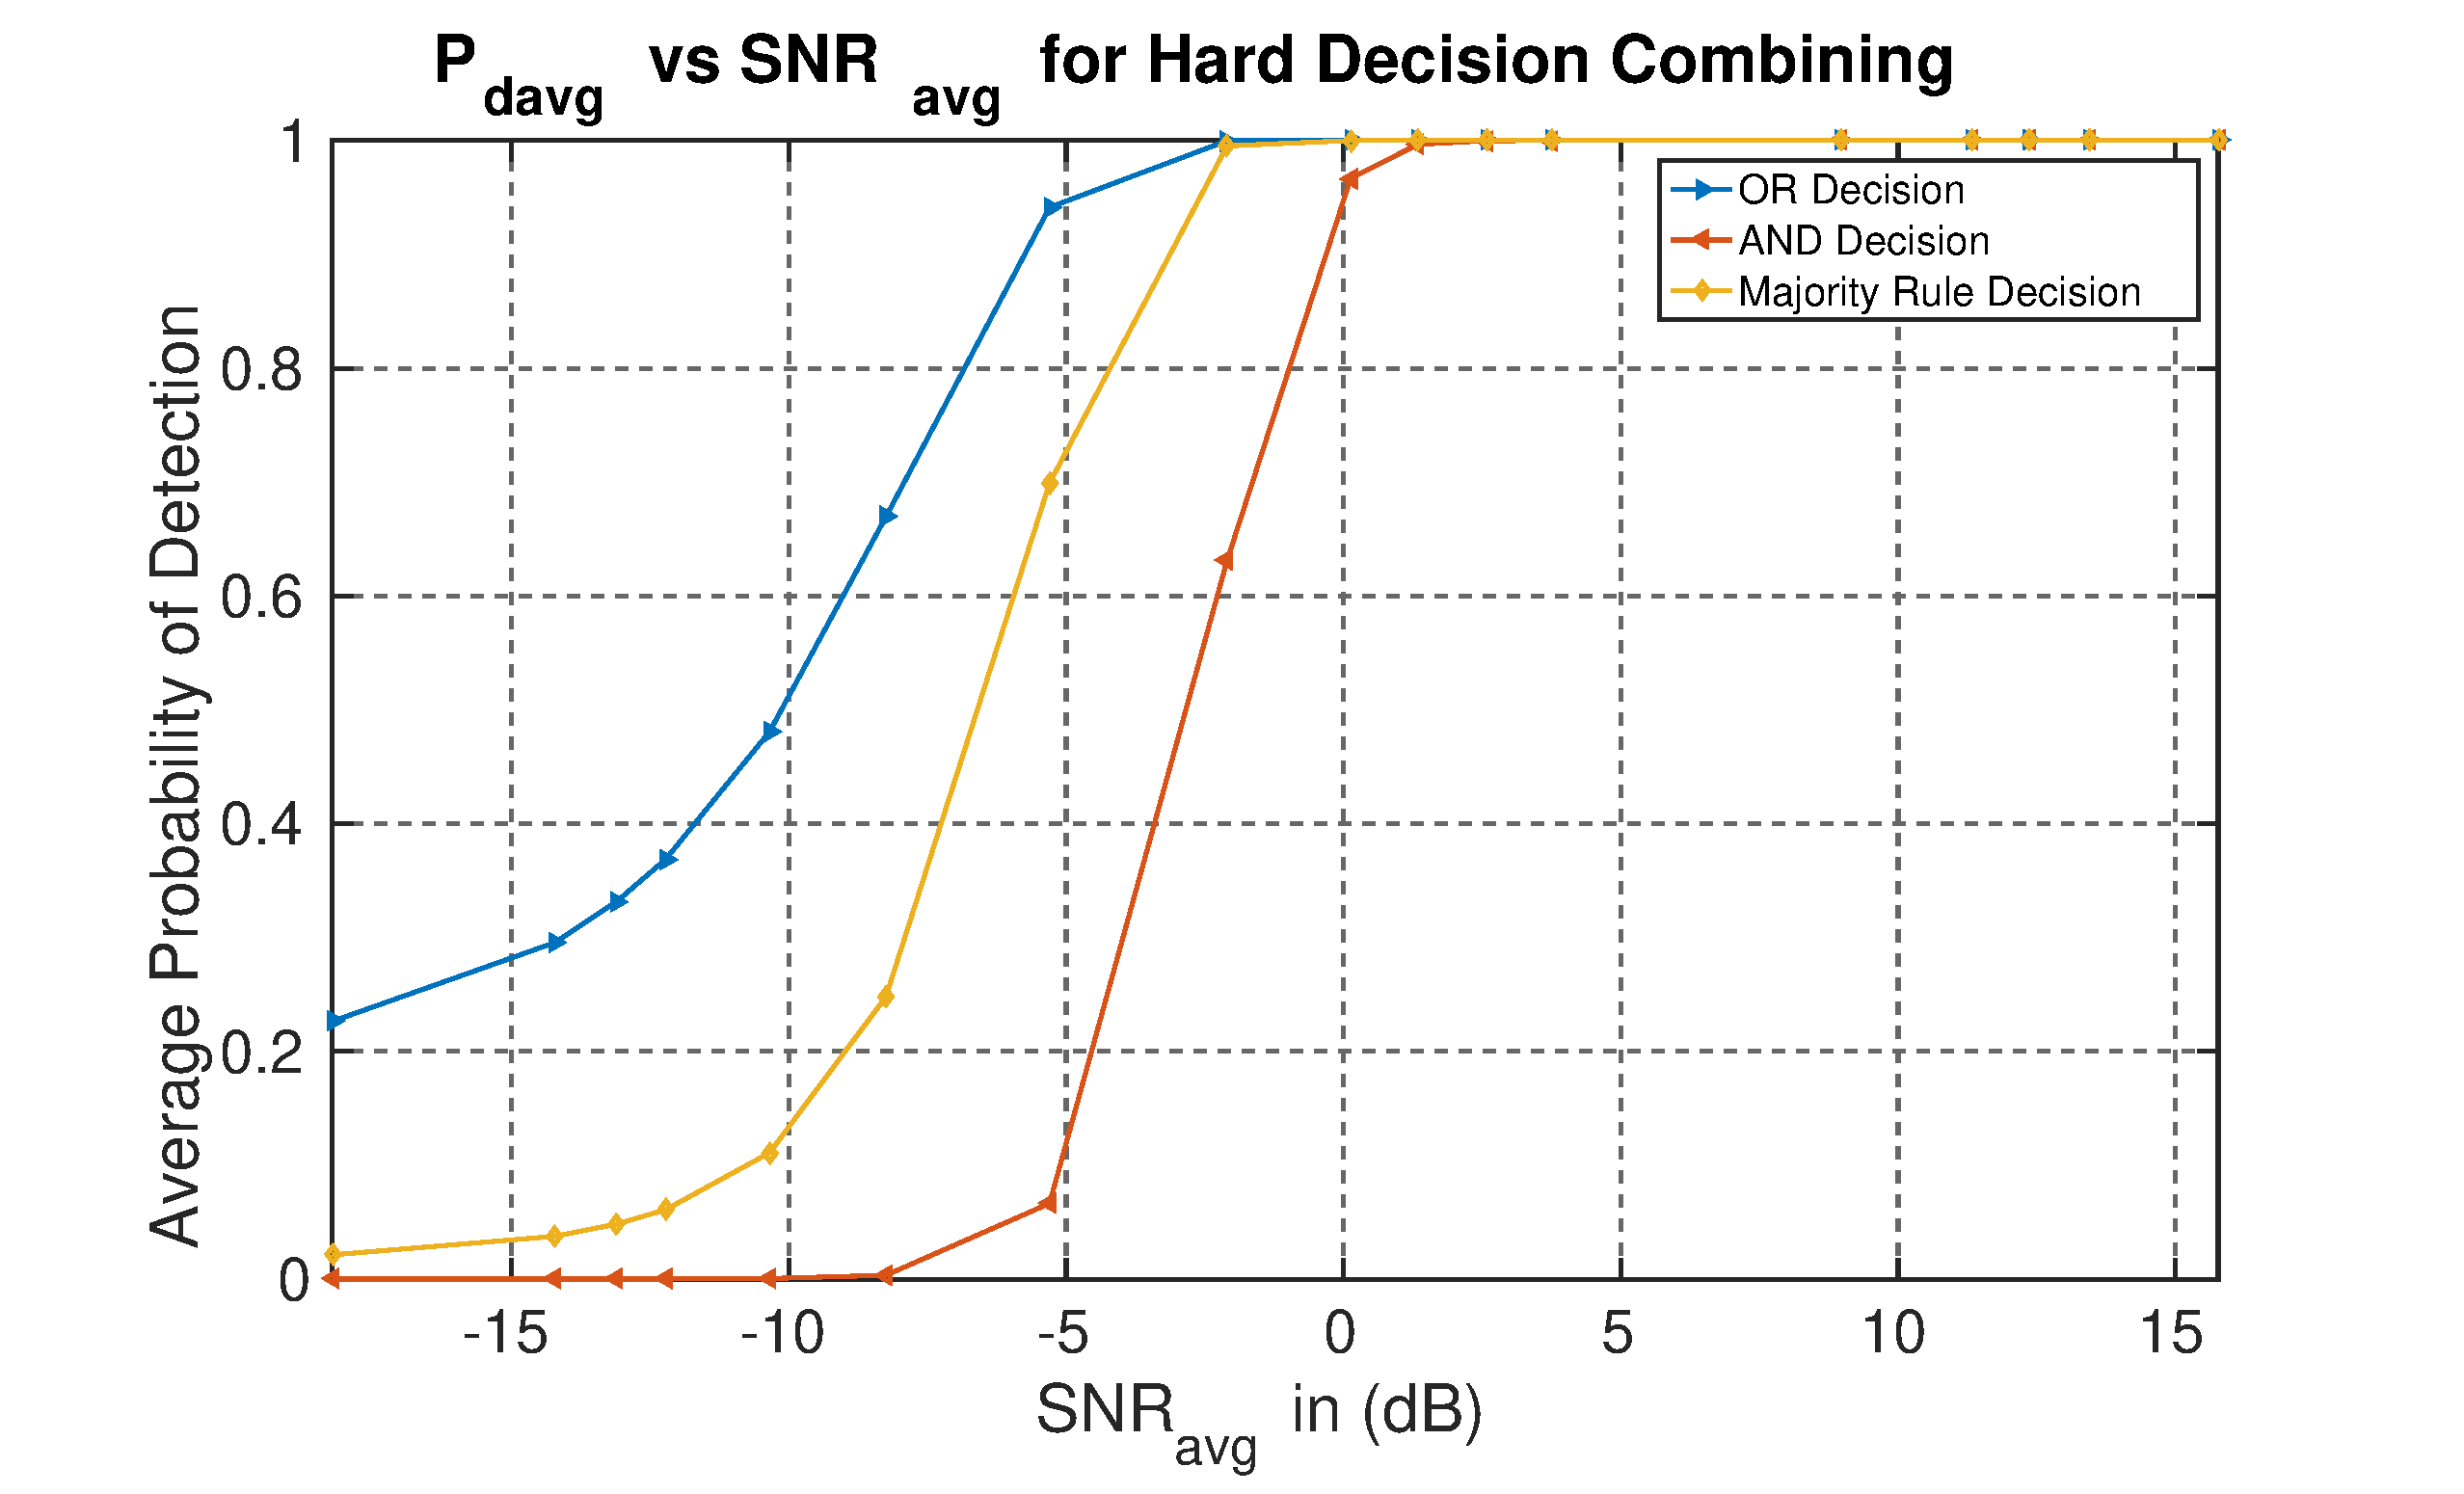
\includegraphics[width=\textwidth,keepaspectratio]{images/Gill/figs/hardecisionpd.eps}
    \caption{Probability of Detection versus $SNR_avg$ For Hard Decision Combining.} 
\label{hardres}      
\end{figure}

\begin{figure}[ht!]
	\centering
	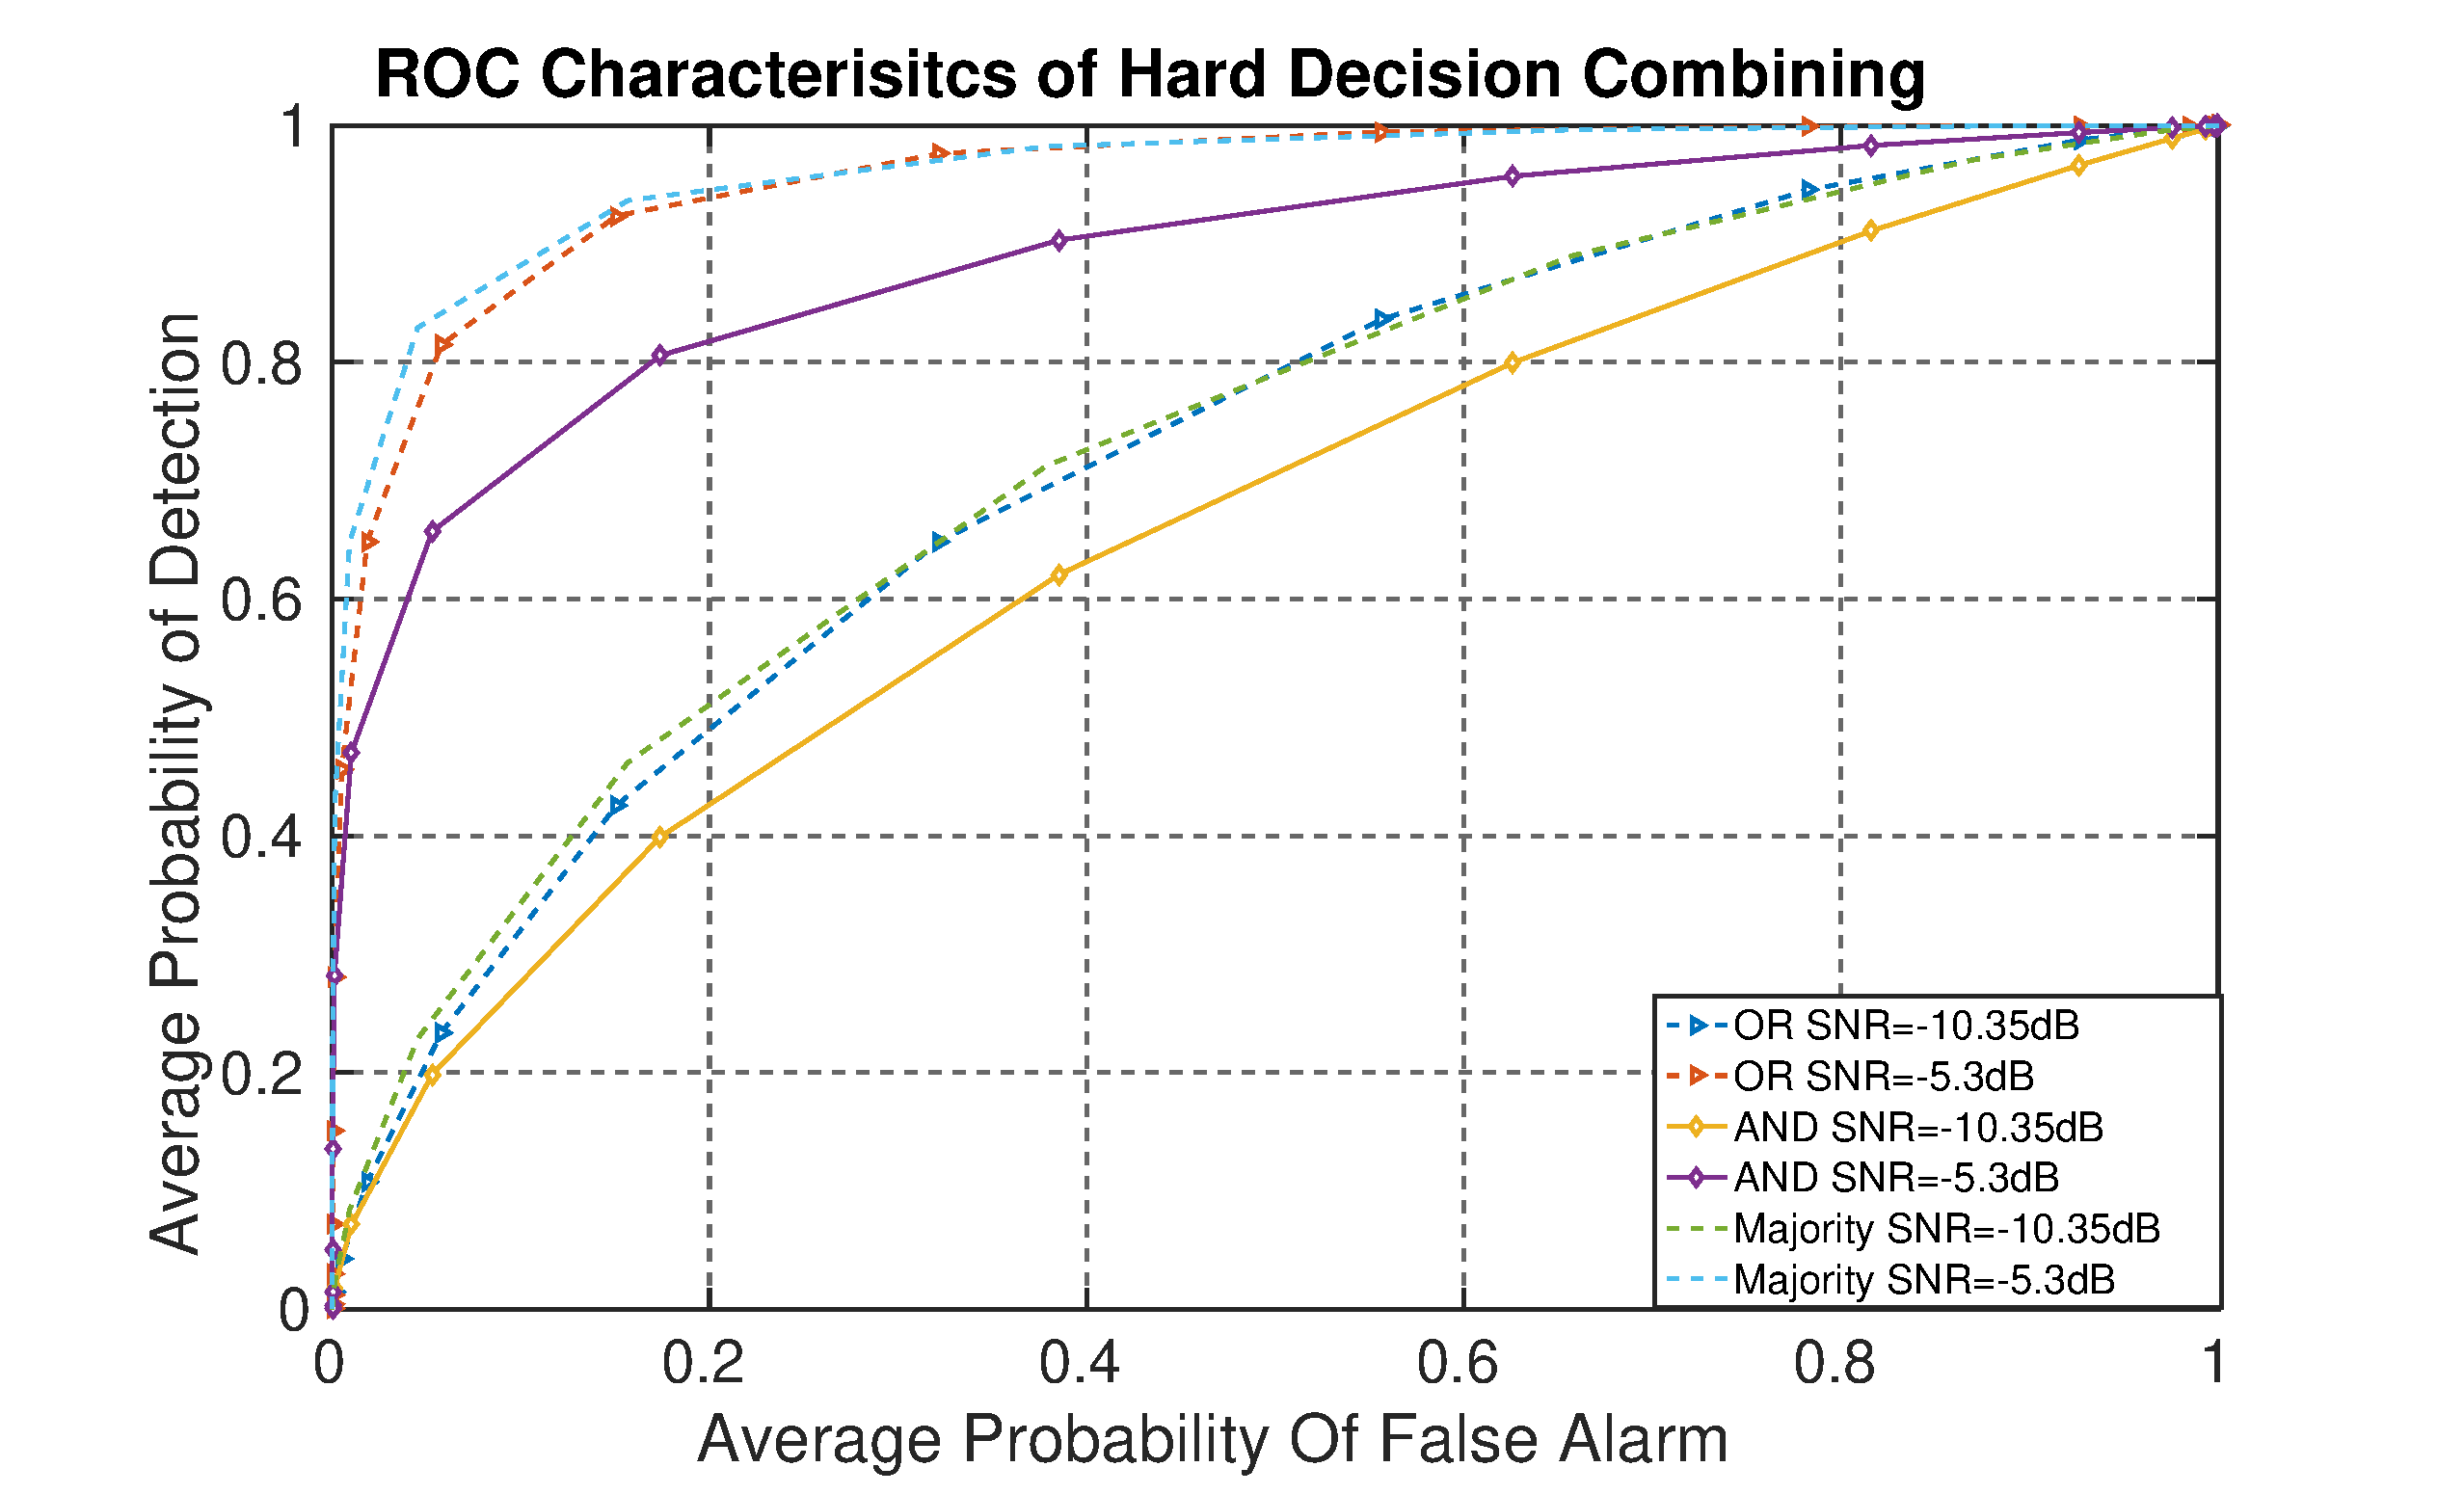
\includegraphics[width=\textwidth,keepaspectratio]{images/Gill/figs/hardecisioroc.eps}
    \caption{ROC Characteristics for Hard Decision Combining with Different SNRs.} 
\label{hardroc}      
\end{figure}

\subsection{Soft Decision Combining}

\begin{figure}[ht!]
	\centering
	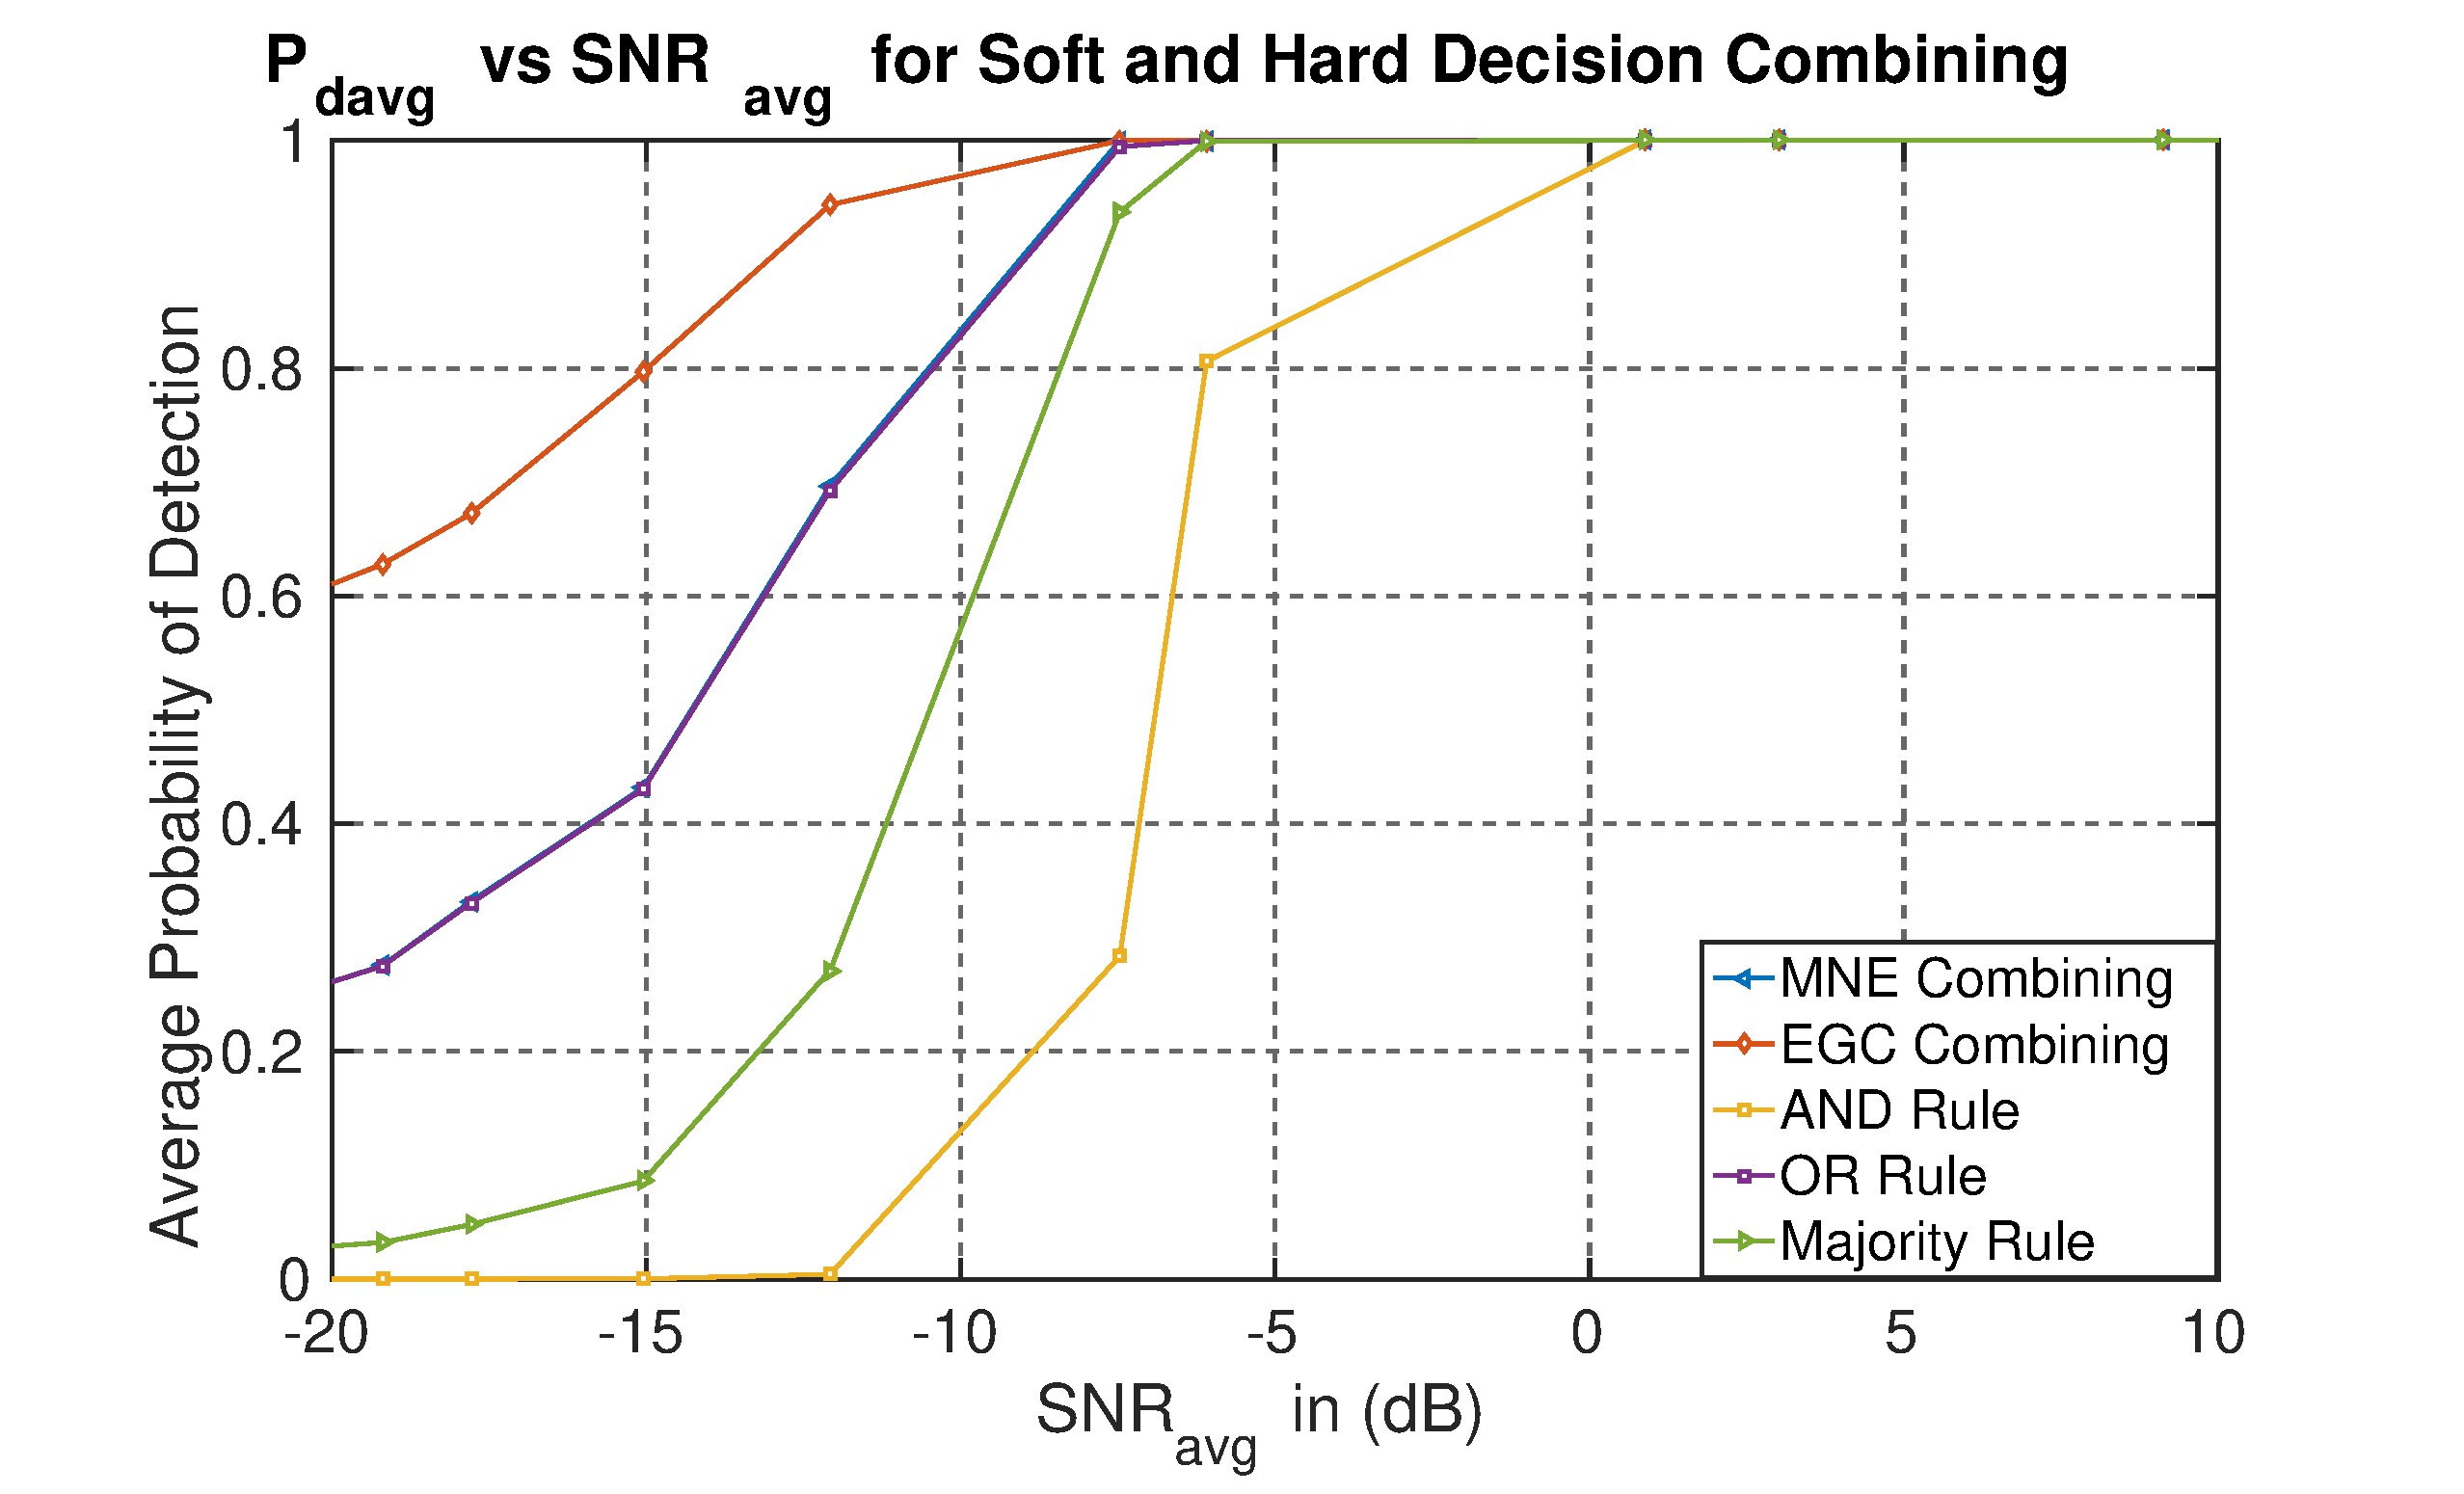
\includegraphics[width=\textwidth,keepaspectratio]{images/Gill/figs/softnhardecisionpd.eps}
    \caption{Probability of Detection versus $SNR_avg$ For Soft and Hard Decision Combining.} 
\label{softpd}      
\end{figure}

\section{HST LTE-R in a Tunnel}

\subsection{K-factor in a Tunnel}

\begin{figure}[!ht]
\label{kfactor}
\centering
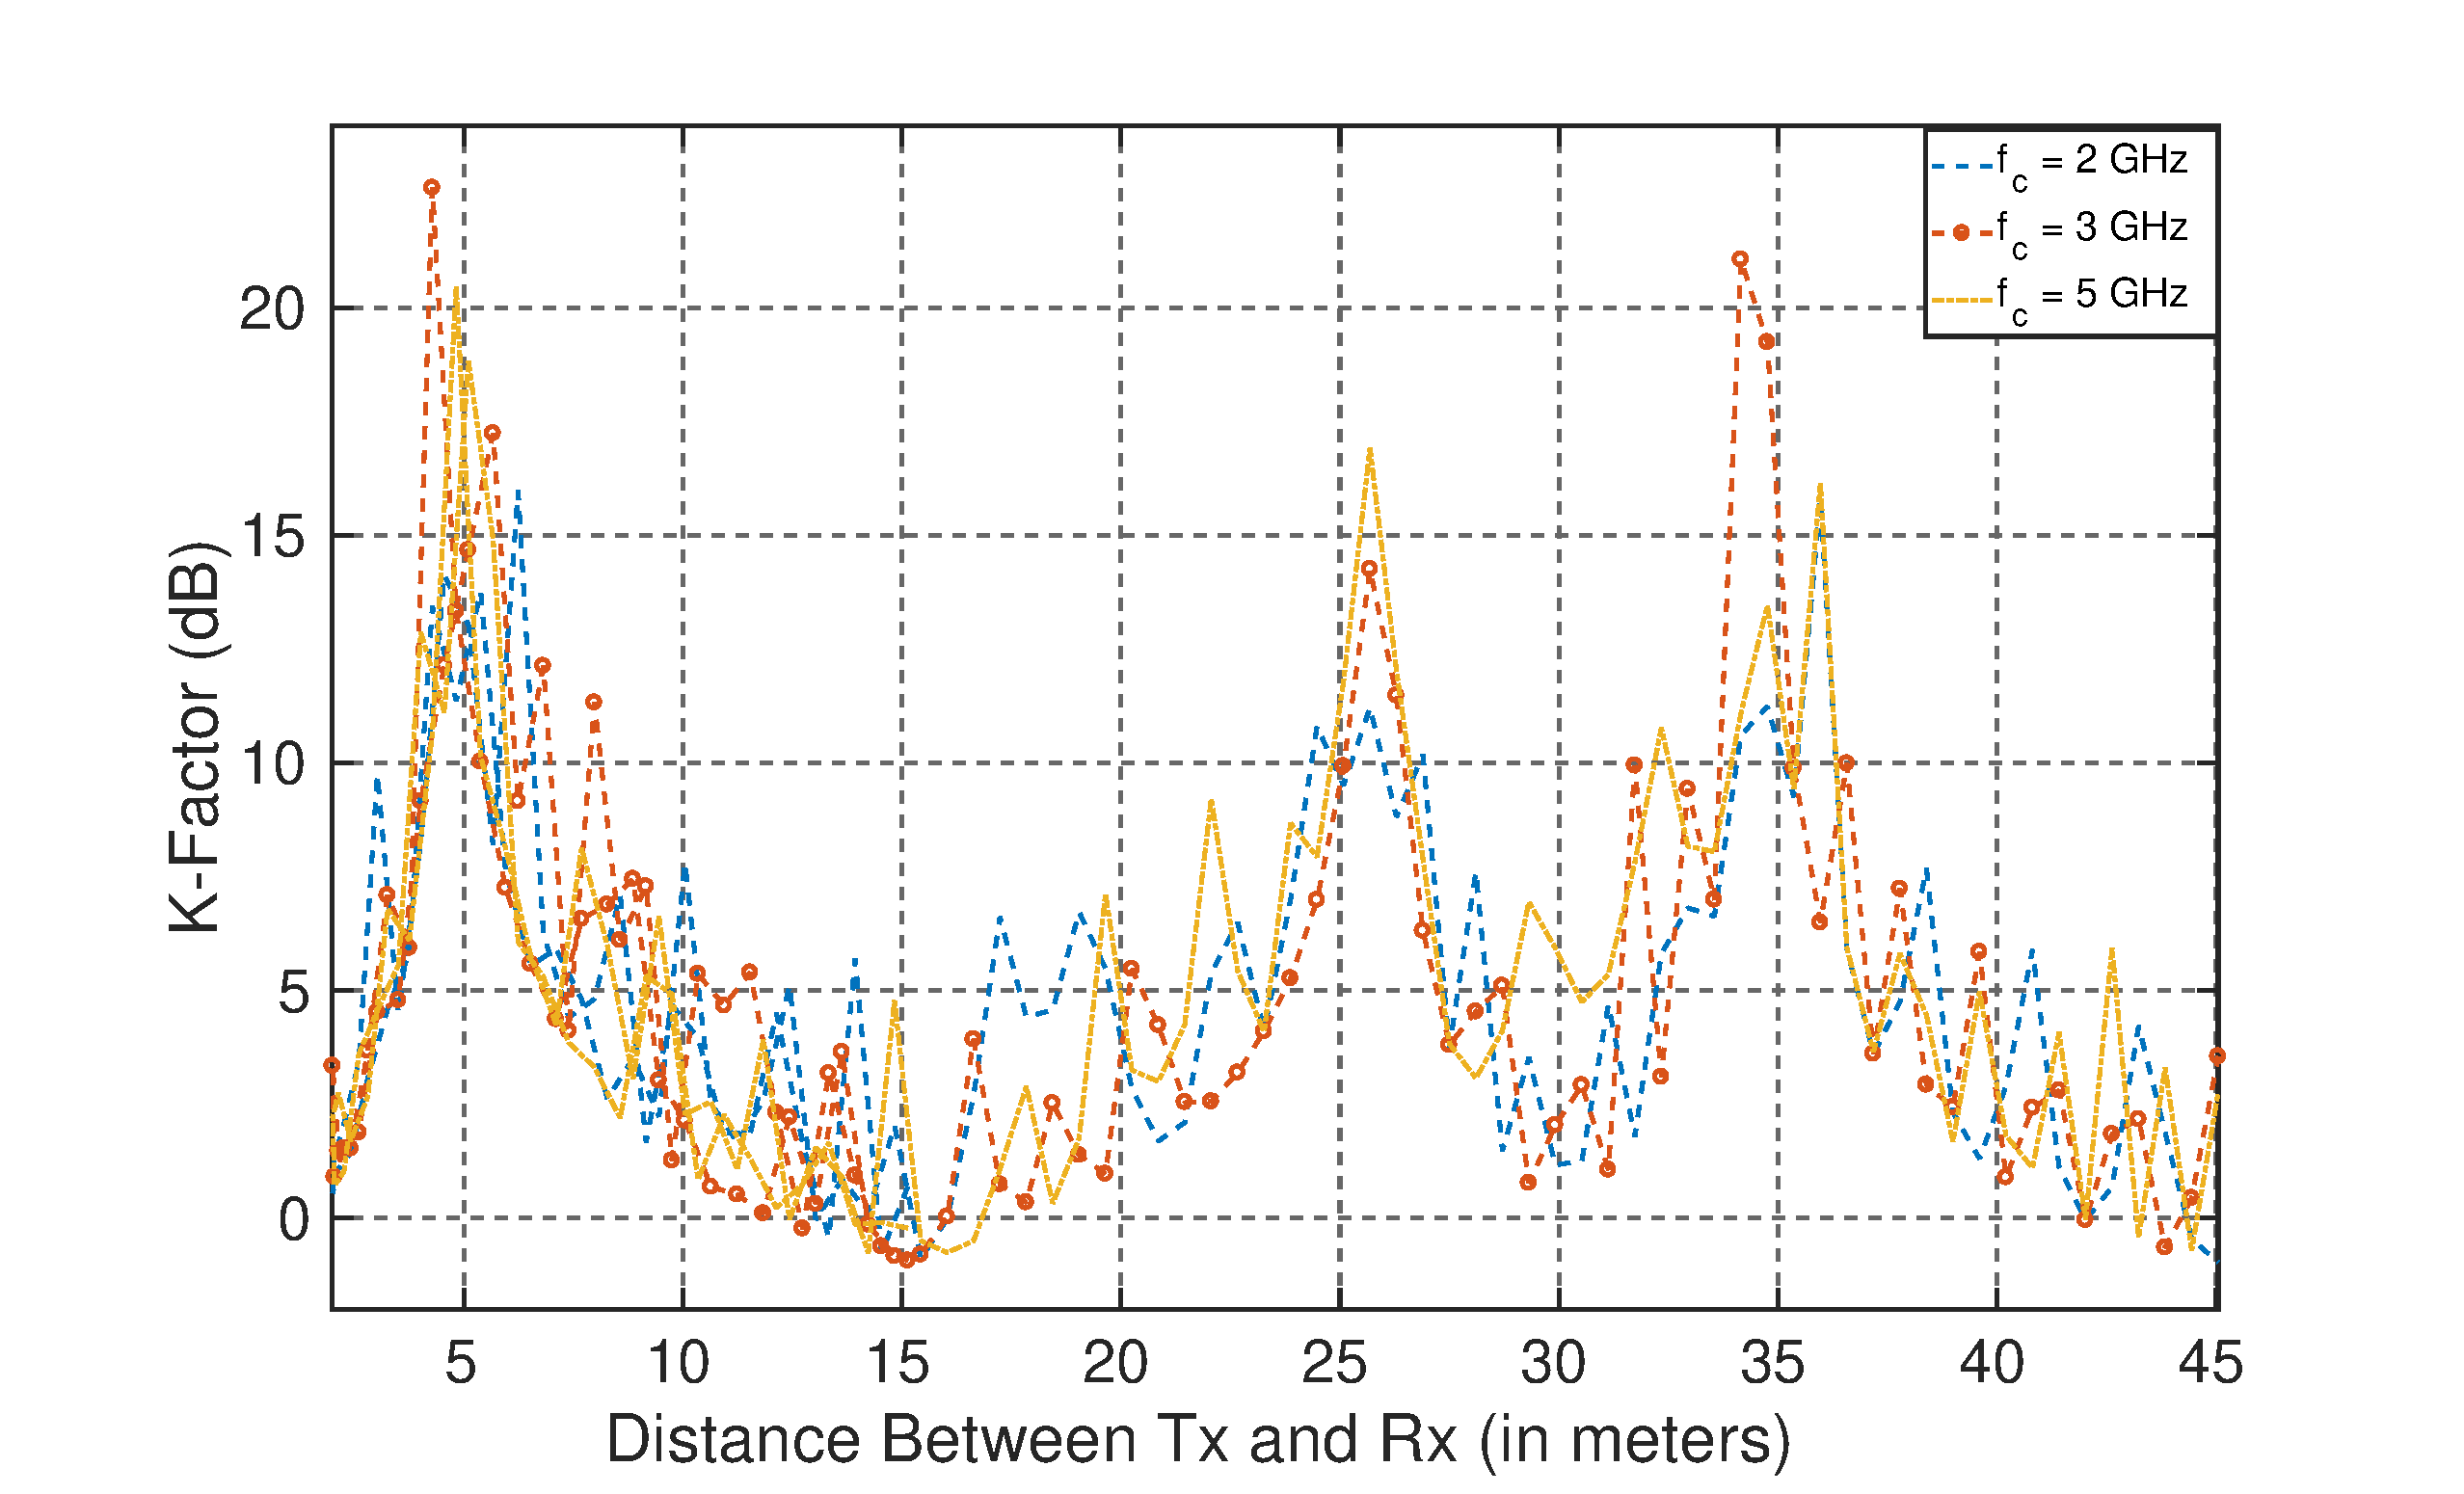
\includegraphics[width=\linewidth,keepaspectratio]{images/Gill/lte_figs/kfactordist.eps} 
\caption{K-factor versus $D_{LOS}$ for different center frequencies $f_c$ = 2, 3 and 5 GHz.}
\end{figure}

\subsection{BER Performance}

\begin{figure}[!ht]
\label{qpsk}
\centering
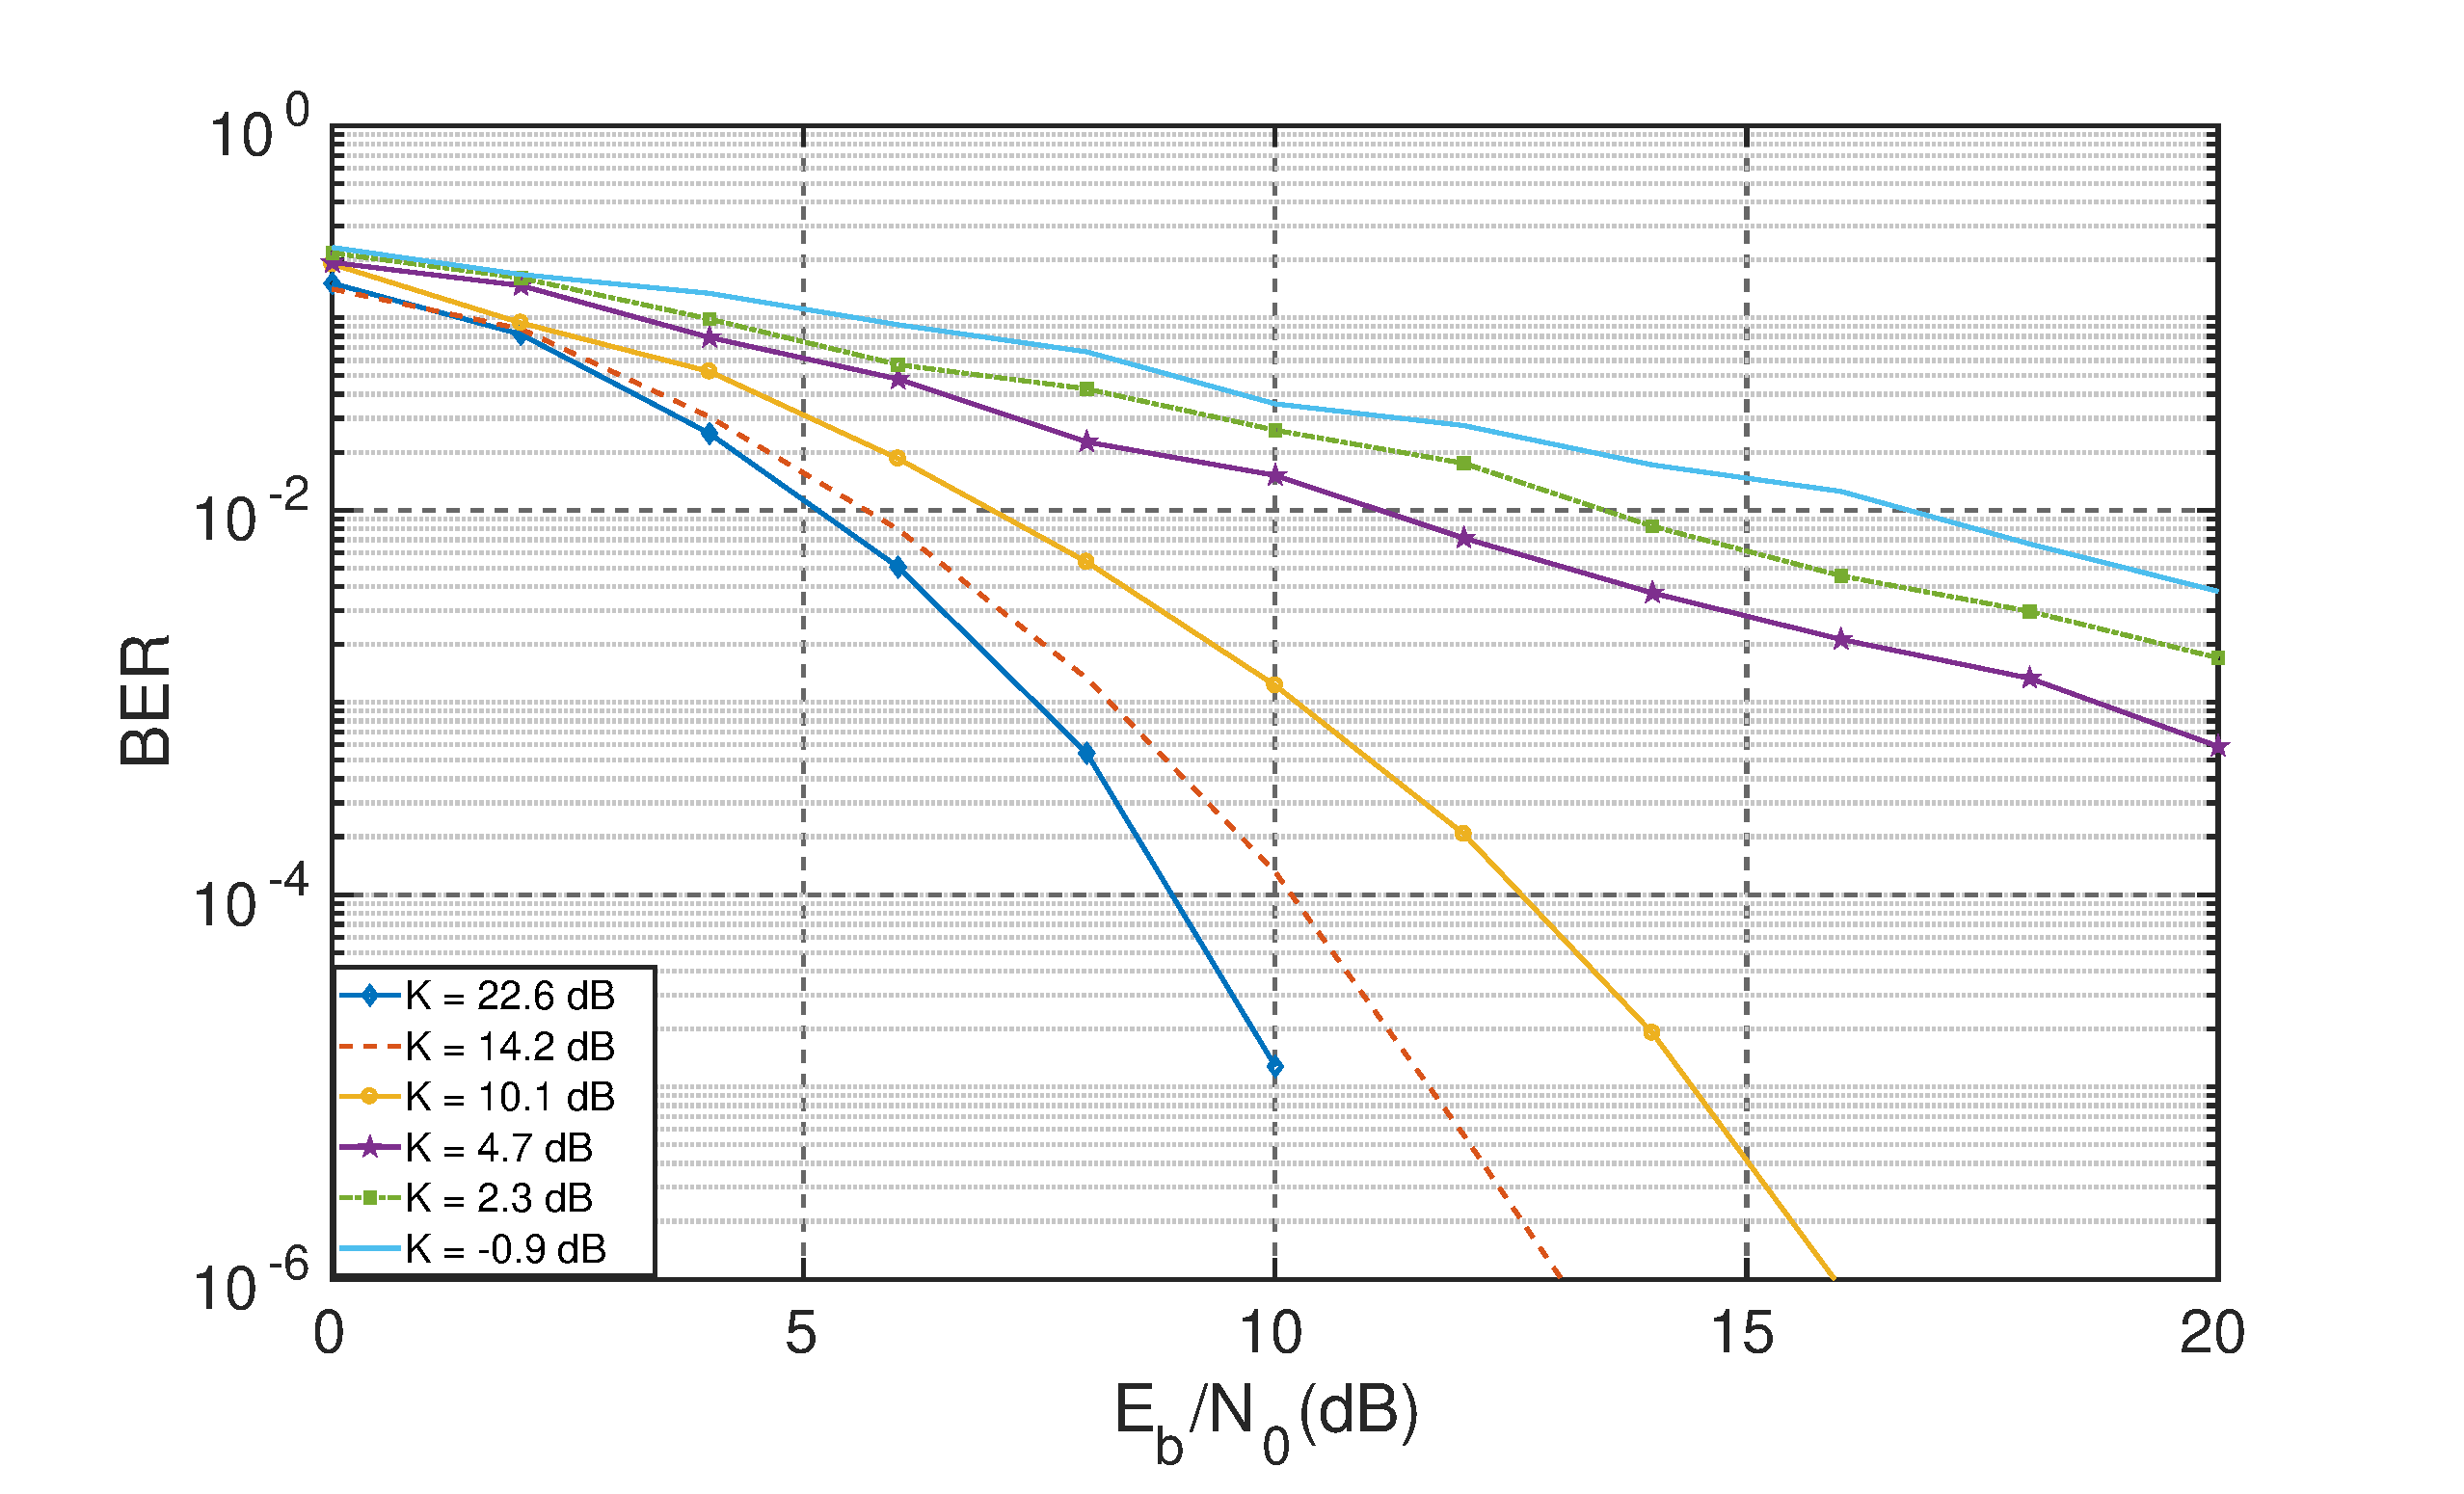
\includegraphics[width=\linewidth,keepaspectratio]{images/Gill/lte_figs/qpskricean.eps} 
\caption{Comparison of $E_b/N_0$ verus BER for LTE-R OFDM-QPSK modulation with different K-factors.}
\end{figure}

\begin{figure}[!ht]
\label{16qam}
\centering
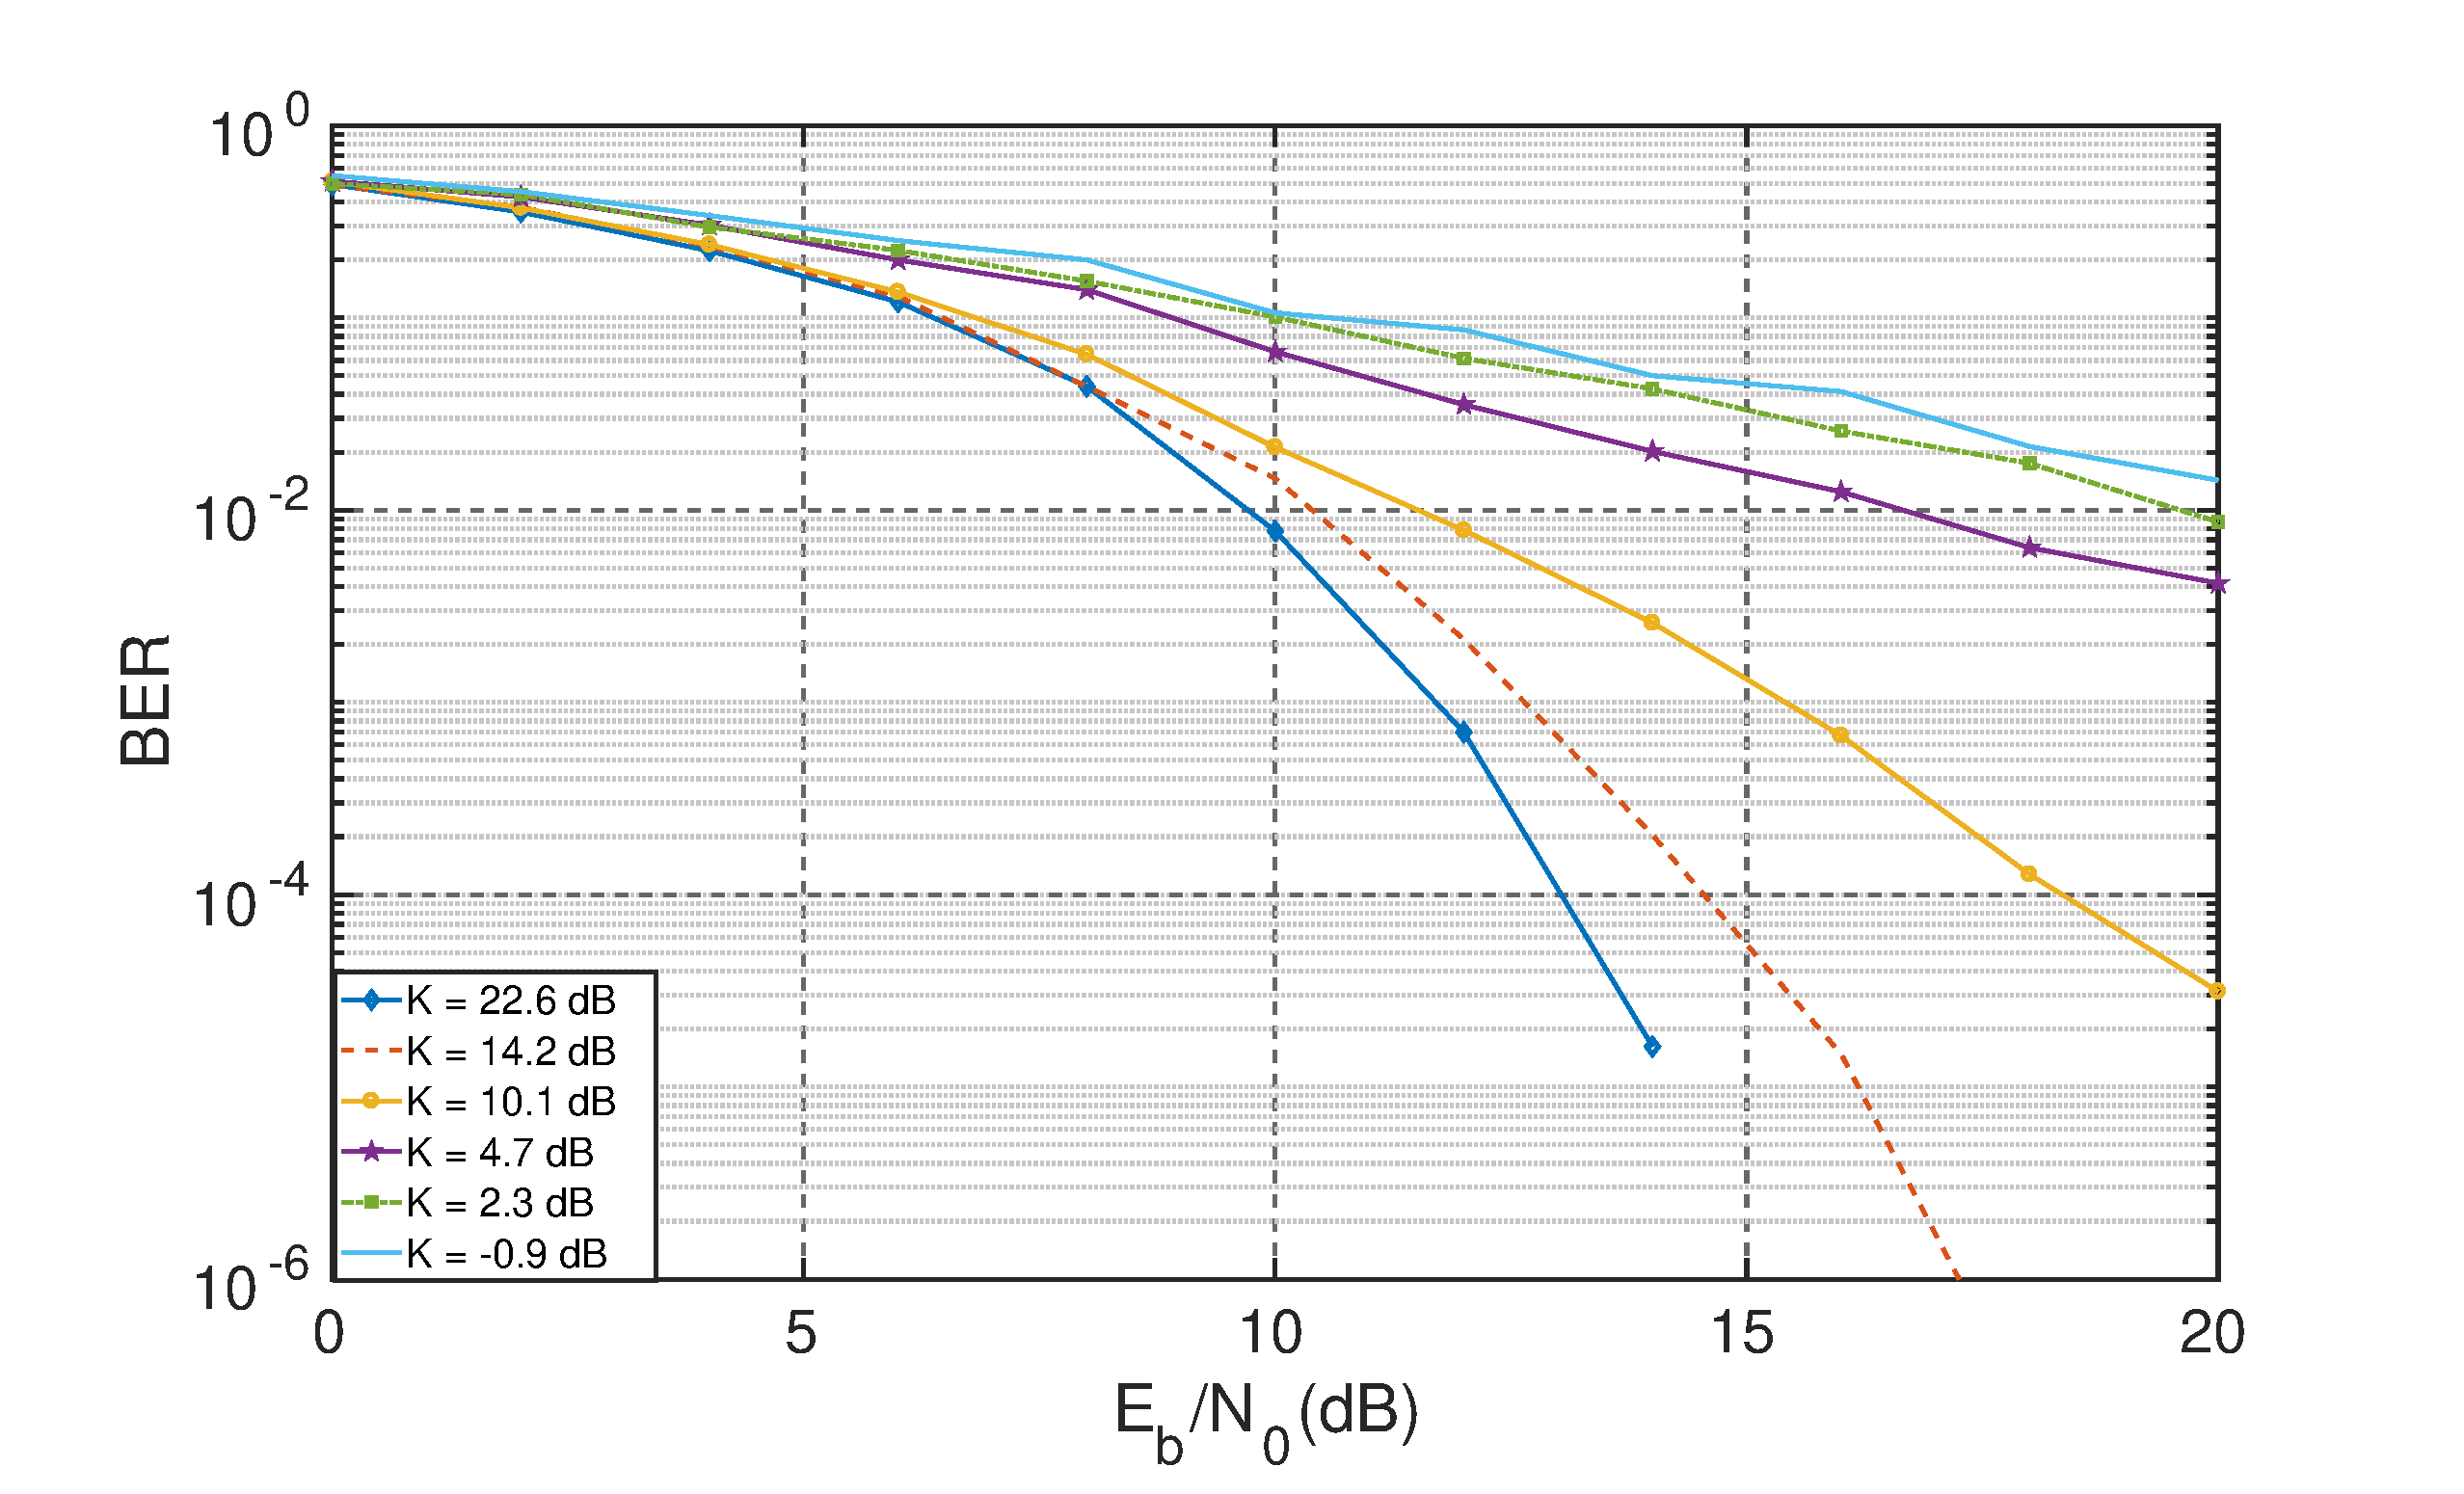
\includegraphics[width=\linewidth,keepaspectratio]{images/Gill/lte_figs/16qamricean.eps} 
\caption{Comparison of $E_b/N_0$ verus BER for LTE-R OFDM-16QAM modulation with different K-factors.}
\end{figure}

\begin{figure}[!ht]
\label{64qam}
\centering
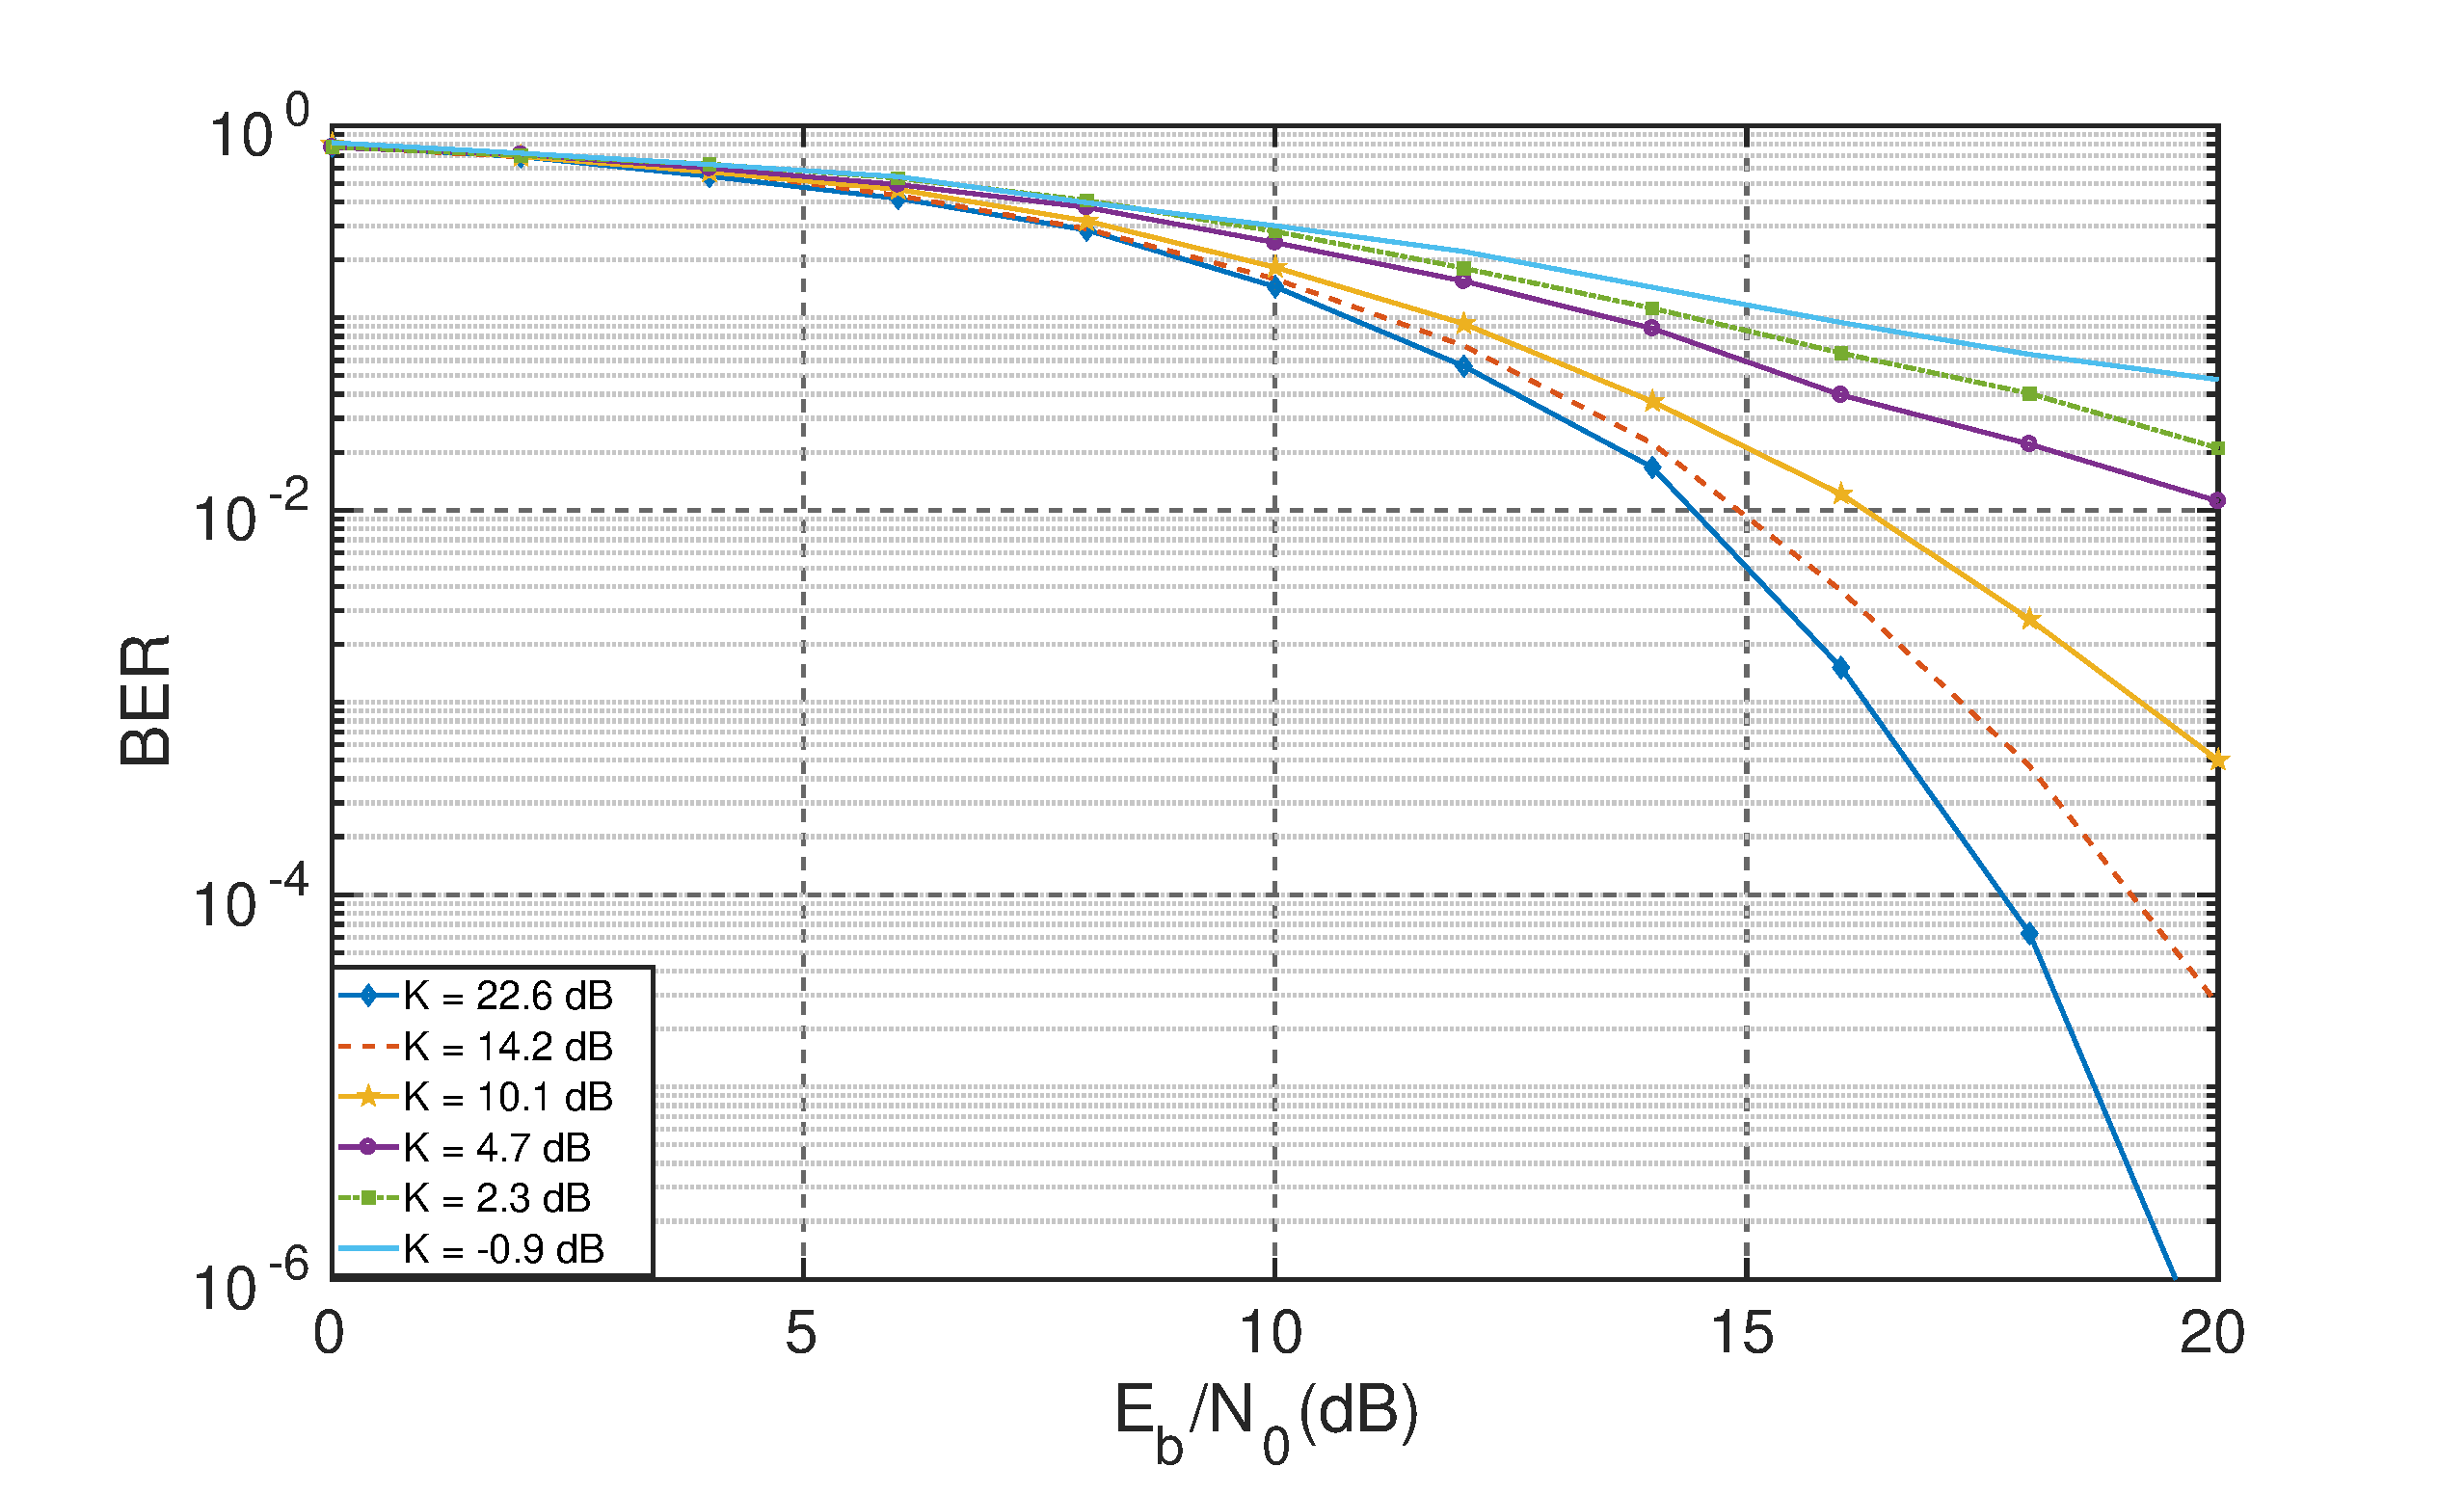
\includegraphics[width=\linewidth,keepaspectratio]{images/Gill/lte_figs/64qamricean.eps} 
\caption{Comparison of $E_b/N_0$ verus BER for LTE-R OFDM-64QAM modulation with different K-factors.}
\end{figure}

\begin{figure}[!ht]
\label{mqam}
\centering
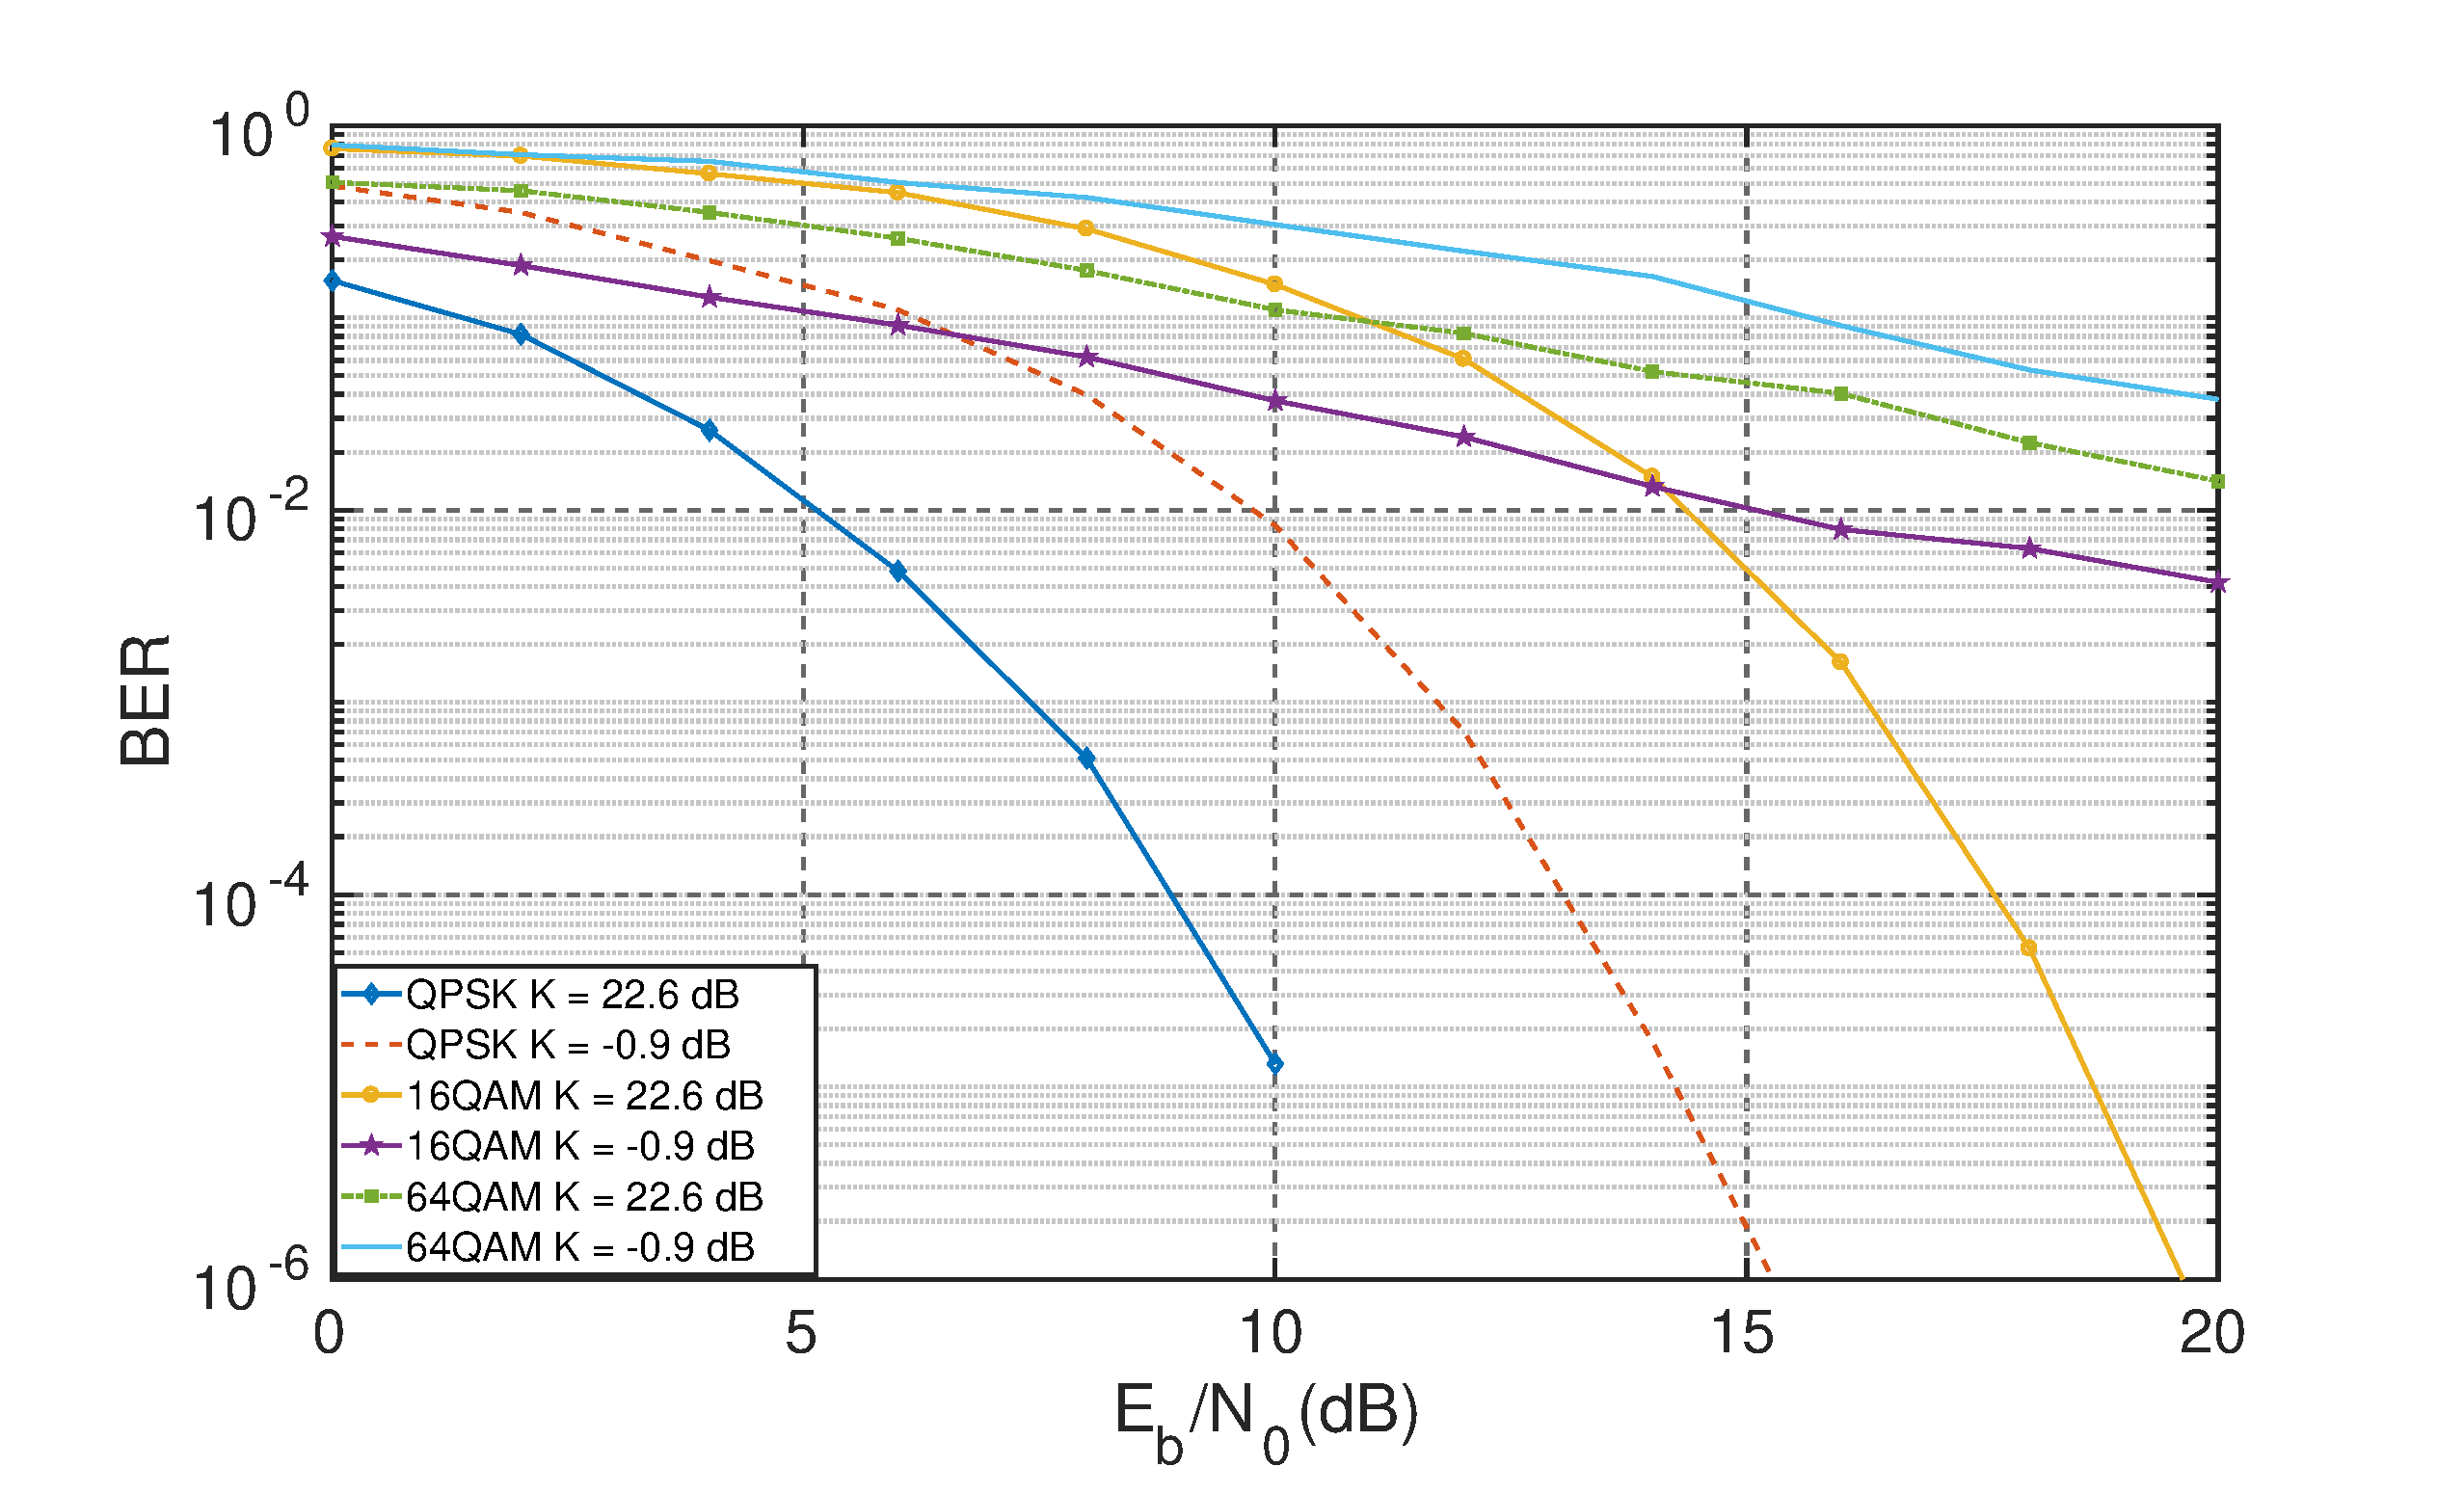
\includegraphics[width=\linewidth,keepaspectratio]{images/Gill/lte_figs/mqamricean.eps} 
\caption{Comparison of $E_b/N_0$ verus BER for LTE-R OFDM modulation with different K-factors.}
\end{figure}


\subsection{Real-time BER in a Tunnel}

\begin{figure}[!ht]
\label{kfactorber}
\centering
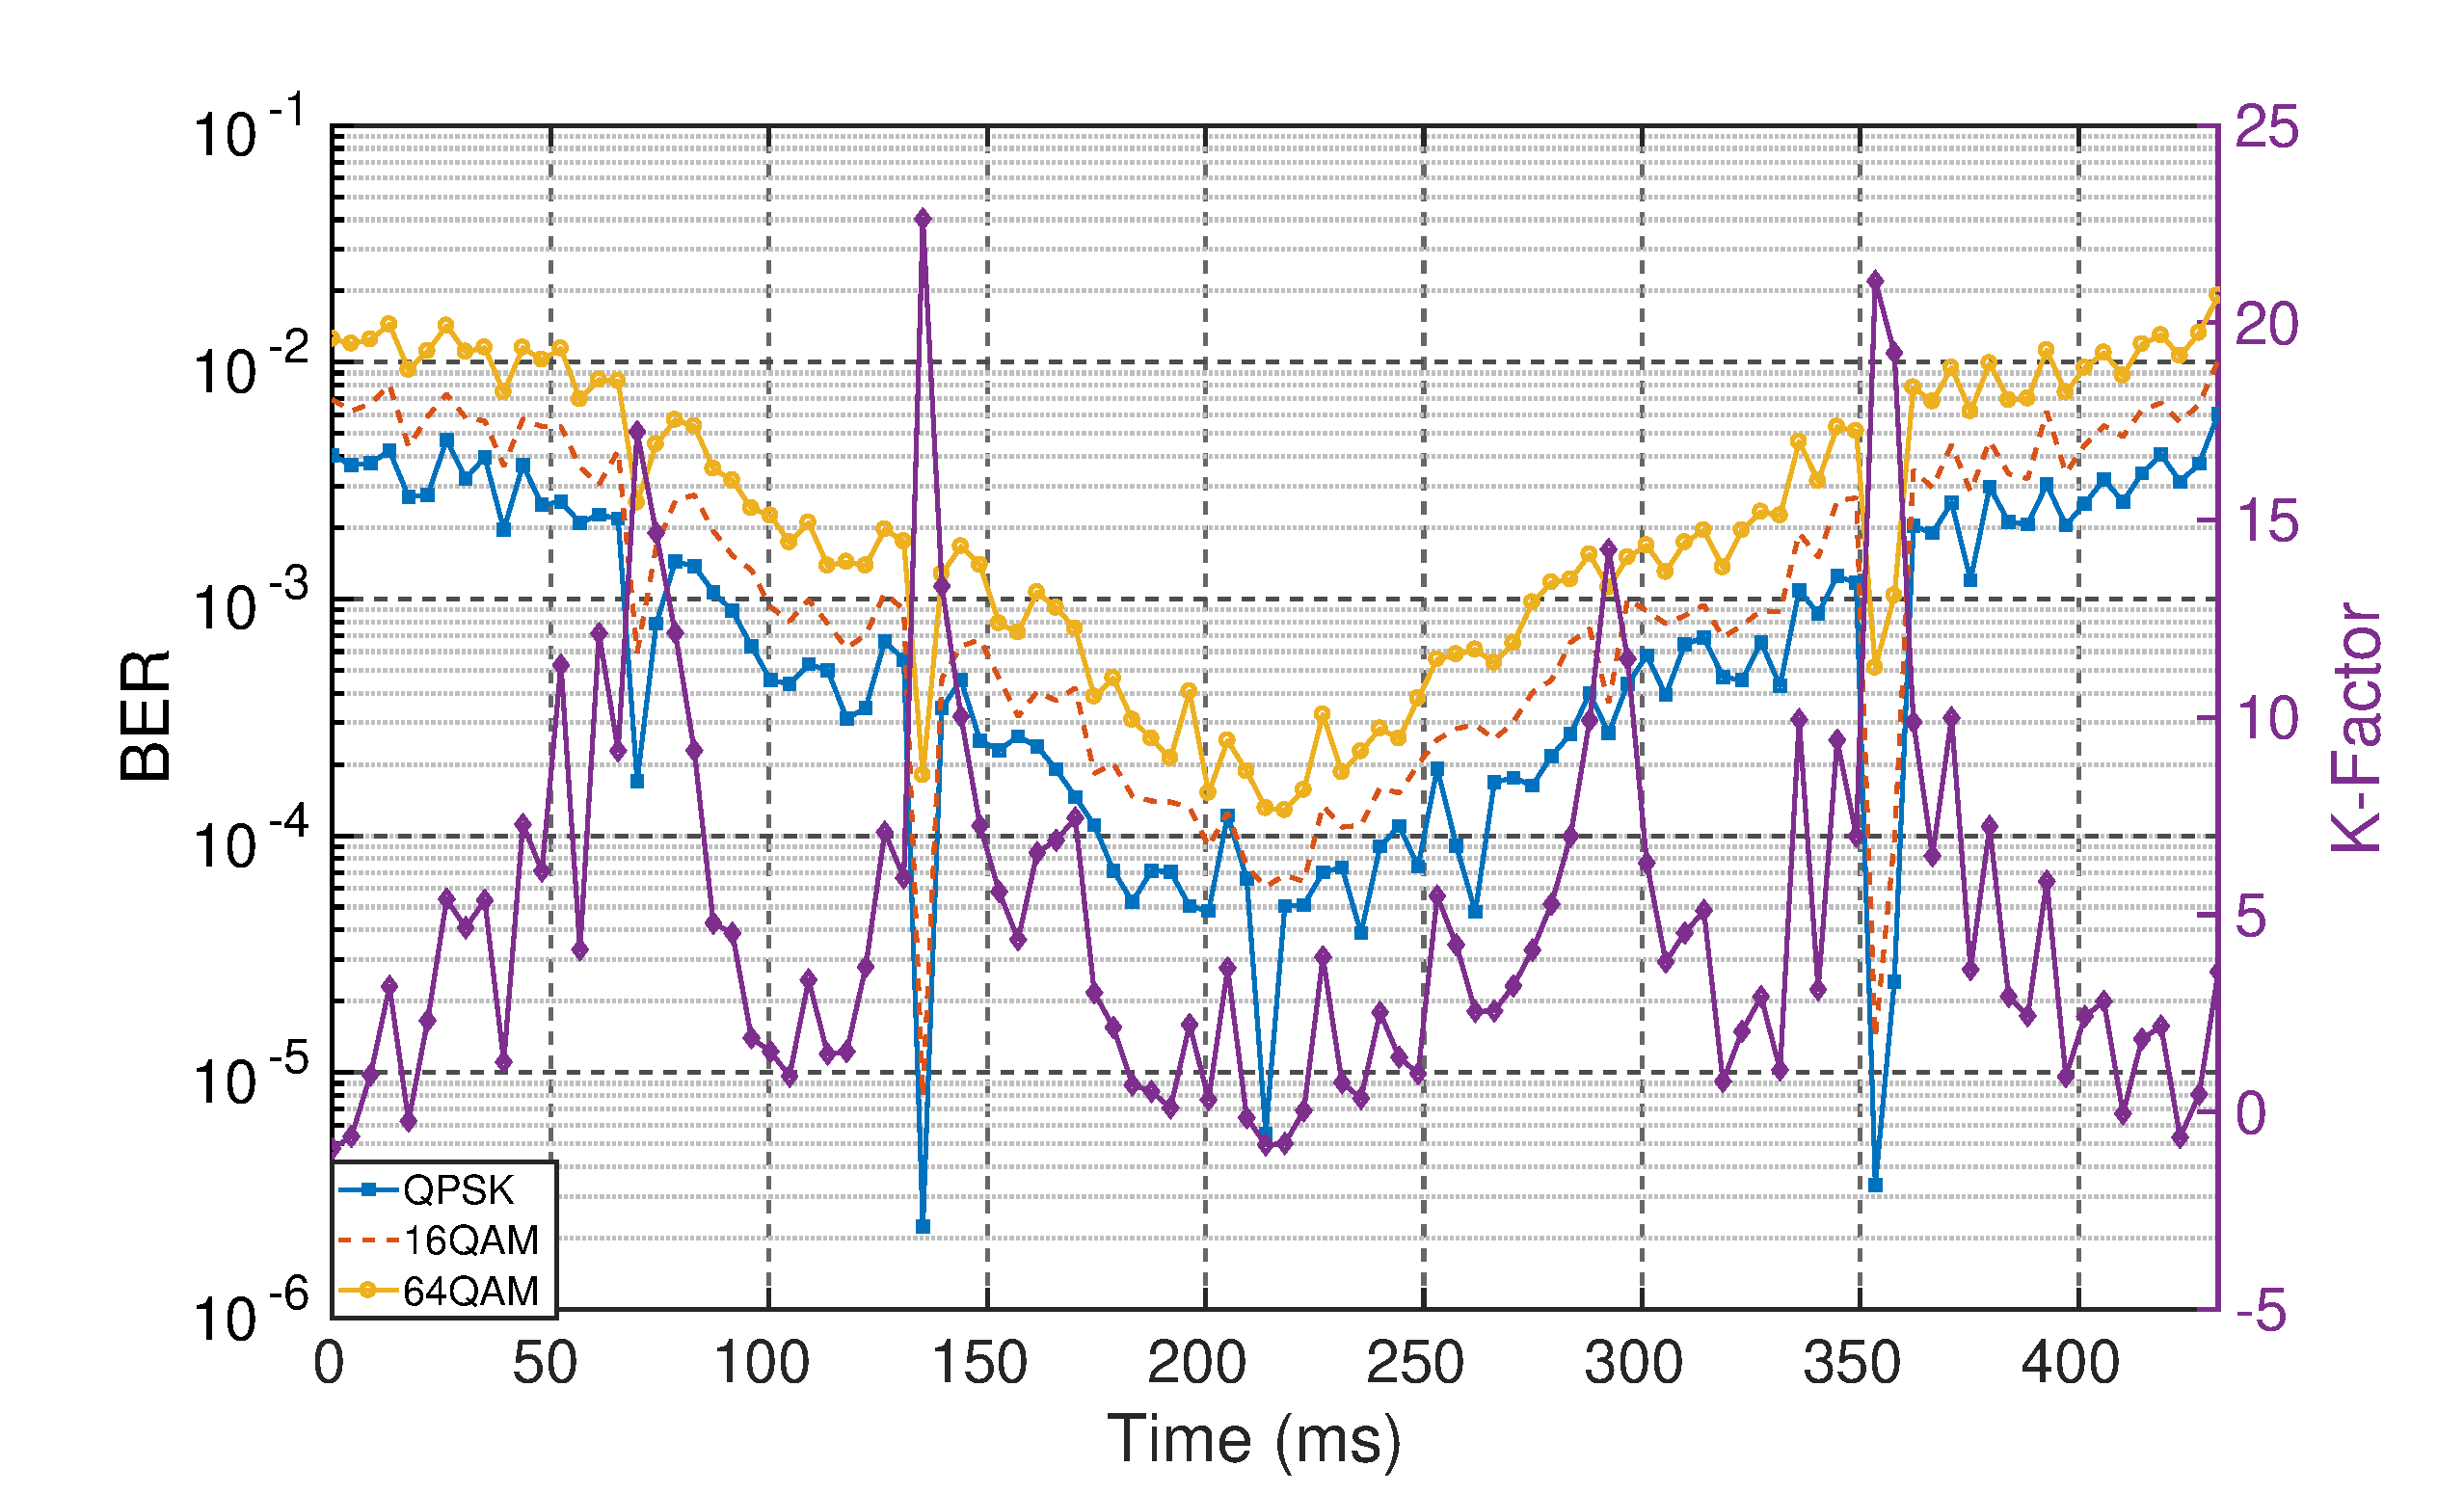
\includegraphics[width=\linewidth,keepaspectratio]{images/Gill/lte_figs/kfactorcontinuous.eps} 
\caption{BER variation with time for HST with different modulation schemes of LTE-R. As the train moves towards
the antenna the general trend of BER goes down with small-scale fluctuations due to varying K-factor.}
\end{figure}




\section{Summary}

Spectral Subtraction in a extremely well studied area in signal processing, but no existing literature exists for its application in a digital communication system.  It has been shown here that it can be quite difficult for it to be applied, even under strict constraints.  Under the conditions of this thesis, the assumptions are quite reasonable, but due to the large amount of error in the results, more may need to be considered.  These may include accuracy requirements for physical equipment, primarily to reduce carrier frequency drift.  Burst scenarios may also be considered to reduce bit error rate.  Overall, for a completely non-existent field of study, these results point the possibility of operational success.  Future work will we required, especially during the implementation phase of designs.\\



